\documentclass[12pt, a4paper]{article}

\usepackage[top=1in, bottom=1in, left=1in, right=1in]{geometry}
%\usepackage{setspace}
%\onehalfspacing
\usepackage{graphicx}
\usepackage{float}

\usepackage{subfig}
\usepackage{amsmath}
\usepackage{url}
\usepackage{listings}
\usepackage{color}
\usepackage{multirow}
\usepackage{url}

\begin{document}

\title{ECE 485 Project \#2}
\author{Jay Mundrawala}
\date{\today}
\maketitle

\begin{abstract}
  This project describes the design and implementation of a multicycle MIPS datapath. Along with it are
  testbenches that issue the appropriate signals for a few signals.
\end{abstract}

\section{Introduction}
The goal of this project was to implement a MIPS datapath capable of executing a small set of instructions.
For this project, we were to implement the following instructions:
\begin{itemize}
  \item LW
  \item SW
  \item ADD
  \item SUB
  \item AND
  \item OR
  \item SLT
  \item BEQ
  \item J
  \item BNE
  \item ADDI
  \item SLL
  \item LUI
  \item JAL
\end{itemize}
The source code for this datapath is available in the appendix and in a git repository on github.
This is available at \url{http://github.com/whois/ECE485_P2}.
\section{Design}
The design for a multicycle MIPS datapath is quite simple. It is shown in Figure \ref{fig:datapath}.
The data path has the following signals
coming from the control unit, which describe how the datapath should operate: PCWrite, IorD, MemRead,
MemWrite, IRWrite, RegDst, MemToReg, RegWrite, ALUSrcA, ALUSrcB, ALUOp, and PCSource. Tables \ref{tbl:1bit} through
\ref{tbl:mtr} enumerate the possible values for these signals and Listings \ref{lst:mipslib} contains their
definitions.

\begin{table}[h]
  \centering
  \begin{tabular}{l | l | l}
    \hline
    Signal name    & Effect when deasserted & Effect when asserted \\ \hline
    PCWrite        & None                   & PC is written \\
    PCWriteCondEq  & None                   & PC is written of zero is asserted \\
    PCWriteCondNEq & None                   & PC is written of zero is deasserted \\
    IorD           & Instruction is Fetched & Data is fetched \\
    MemRead        & None                   & Memory at given address is read \\
    MemWrite       & None                   & Data is written to given address \\
    IRWrite        & None                   & Instruction register is written \\
    RegWrite       & None                   & Data is written to register \\
    ALUSrcA        & Port A of ALU gets PC  & Port A of ALU gets register A's output \\
    \hline
  \end{tabular}
  \caption{Actions of 1-bit control signals}
  \label{tbl:1bit}
\end{table}

\begin{table}[h]
  \centering
  \begin{tabular}{l | l} \hline
    \multicolumn{2}{c}{ALUSrcB} \\ \hline
    Signal value & Effect \\ \hline
    ASB\_REGB & Port B of ALU gets register B's output \\
    ASB\_FOUR & Port B of ALU gets $4$ \\
    ASB\_SEXT & Port B of ALU gets instruction[15-0] sign extended to 32 bits \\
    ASB\_SEXTS & Same as previous except value is shifted left by 2 \\
    \hline
  \end{tabular}
  \caption{Actions of ALUSrcB signal}
  \label{tbl:alusrcb}
\end{table}

\begin{table}[h]
  \centering
  \begin{tabular}{l | l} \hline
    \multicolumn{2}{c}{ALUOp} \\ \hline
    Signal value & Effect \\ \hline
    AOP\_AND & ALU will 'and' the two operands \\
    AOP\_OR  & ALU will 'or' the two operands \\
    AOP\_ADD & ALU will add the two operands \\
    AOP\_SUB & ALU will subtract A - B \\
    AOP\_SLT & ALU will output '1' if $A<B$, '0' otherwise \\
    AOP\_NOR & ALU will NOR the two operands \\
    AOP\_SLL & ALU will shift B left by instruction[10-6] \\
    \hline
  \end{tabular}
  \caption{Actions of ALUOp signal}
  \label{tbl:aluop}
\end{table}

\begin{table}[h]
  \centering
  \begin{tabular}{l | l} \hline
    \multicolumn{2}{c}{PCSource} \\ \hline
    Signal value & Effect \\ \hline
    PS\_PCINC    & Value to PC is $PC+4$ \\
    PS\_ALUOUT   & Value to PC is that of the register ALU OUT \\
    PS\_JMP      & Value to PC is $PC[31-28] + Instr[25-0] << 2$ \\
    \hline
  \end{tabular}
  \caption{Actions of PCSource signal}
  \label{tbl:pcSrc}
\end{table}

\begin{table}[h]
  \centering
  \begin{tabular}{l | l} \hline
    \multicolumn{2}{c}{RegDst} \\ \hline
    Signal value & Effect \\ \hline
    RD\_RT       & Write register is set to instr[25-21] \\
    RD\_RD       & Write register is set to instr[20-16] \\
    RD\_RA       & Write register is set to $R31$ \\
    \hline
  \end{tabular}
  \caption{Actions of RegDst signal}
  \label{tbl:regDst}
\end{table}

\begin{table}[h]
  \centering
  \begin{tabular}{l | l} \hline
    \multicolumn{2}{c}{MemToReg} \\ \hline
    Signal value & Effect \\ \hline
    MTR\_ALUOUT  & Register write data gets the output of the ALU OUT register \\
    MTR\_MDR     & Register write data gets the output of the MDR register \\
    MTR\_PC      & Register write data gets the PC \\
    \hline
  \end{tabular}
  \caption{Actions of MemToReg signal}
  \label{tbl:mtr}
\end{table}

\begin{figure}[ht]
  \centering
  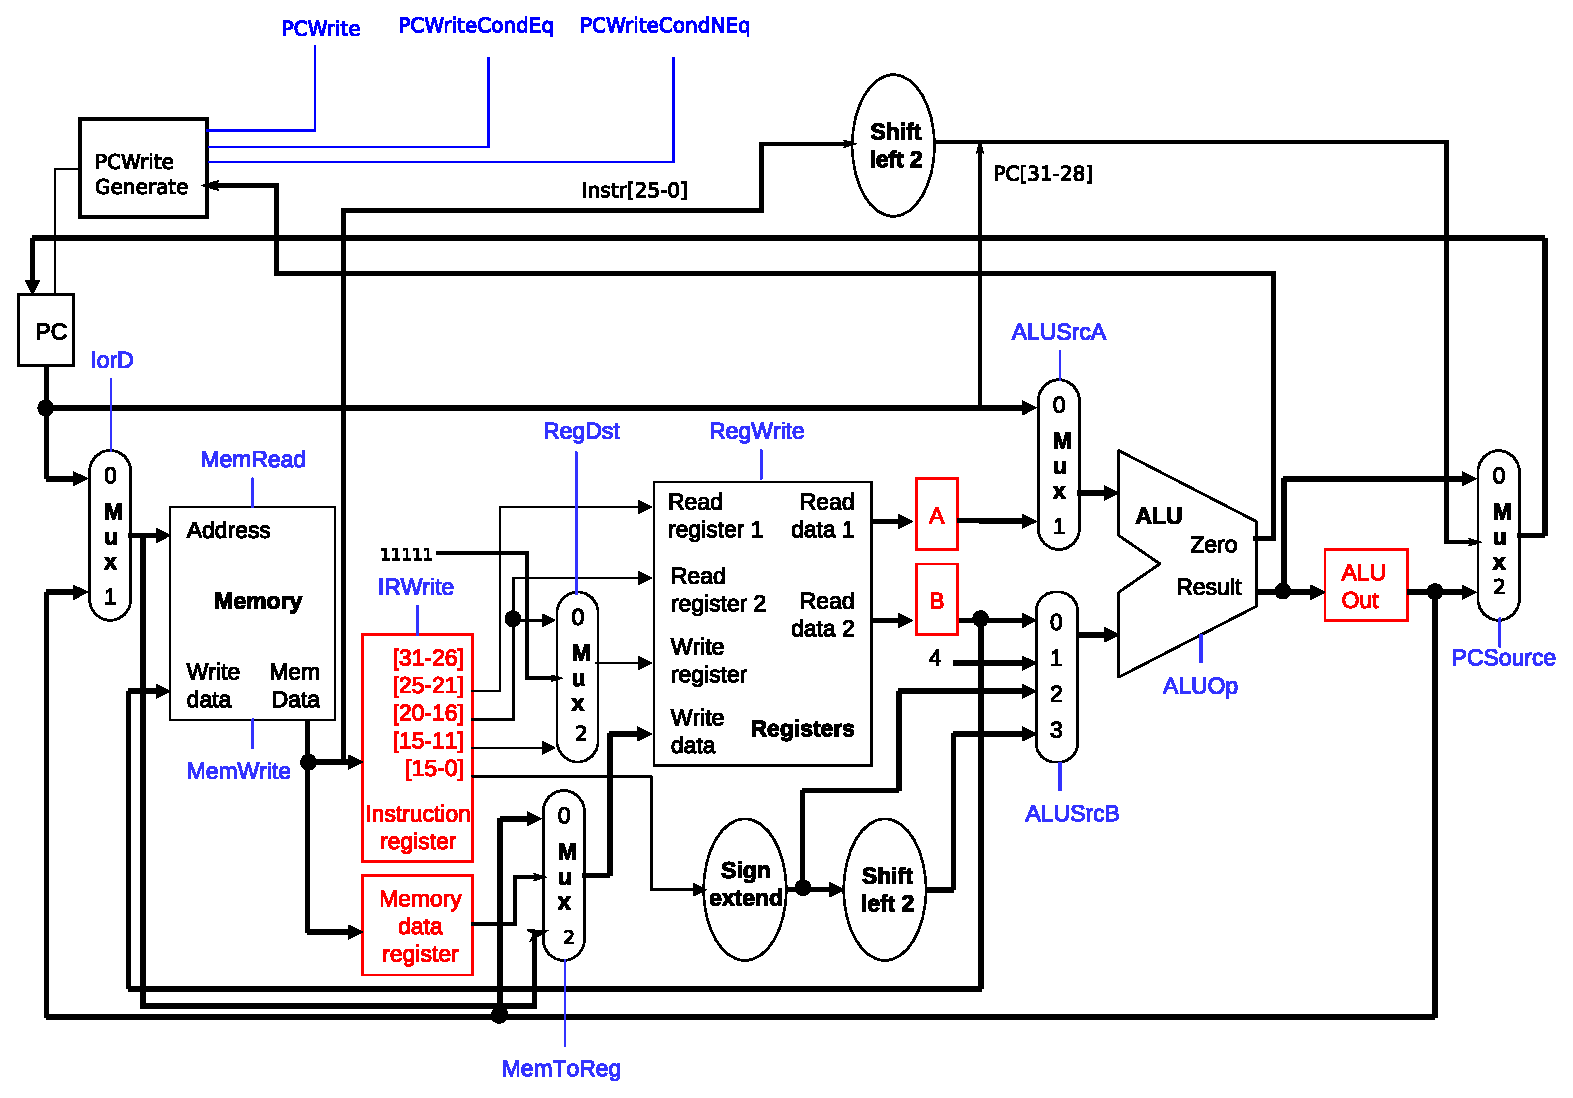
\includegraphics[width=6in]{images/datapath.eps}
  \caption{MIPS multicycle datapath}
  \label{fig:datapath}
\end{figure}

With these signals defined, we can begin by defining each functional block in Figure \ref{fig:datapath}.
First, we have the PC. This is the program counter and stores the address of the next instruction to be
executed. The memory block is our RAM. For this project, the test benches only output one value when the
memory is read, and that is the instruction we are testing. This allows us to test the datapath without
creating a memory module. Nothing is ever written to the memory; when testing LW we analyze the value on
the write data line when it is time to write to the memory. The instruction register holds the values
of the instruction being executed. The memory data register(MDR), stores the value read from memory. This
will be written every clock cycle since the value only need be stored for one clock cycle. Thus, it does
not need its own control signal and its enable can be attached to the clock. The register file, denoted by
Registers in Figure \ref{fig:datapath}, stores the 32 registers. Register A and B store the output of
the register file for one clock cycle. The ALU does all the arithmetic computations. Its functionality
is fully described by Table \ref{tbl:aluop}. The ALU OUT register holds the output of the ALU for one
clock cycle. PCWrite Generate generates the enable signal to write to the PC. In the case of this design,
it is described by the following equation: 
$G = PCWrite + PCWriteCondEq*zero + PCWriteCondNEq*\overline{zero}$.

\subsection{Instruction Fetch, Instruction Decode, and Branch Target Computation}
There are two steps that each instruction execution has in common. The first is the IF stage. Each
instruction needs to be fetched from memory. To do this, we need to read the instruction from memory
and store it into the instruction register. This is also the step where we must update the PC to $PC+4$.
So, with that in mind, we can define the signals needed to complete this step. First, IorD needs to be
deasserted. This will select the PC as the address for memory. MemRead needs to be set, so that the
instruction is fetched from memory. IRWrite needs to be asserted so that the instruction is stored 
after it is read. This is enough to actually fetch the instruction, but the PC still needs to be updated.
Thus, we require ALUSrcA to be deasserted to select PC for port A of the ALU, and ALUSrcB to be set
to ASB\_FOUR to select 4 for the second port($PC+4$). PCSource needs to be set to PS\_PCINC inidcating
that $PC+4$ should be written to the PC. Finally, PCWrite needs to be asserted so that the value is
written to the PC. One thing that should be noted is that all writes happen only when the clock is high,
except for the IRWrite. This is a bug, however it does not affect the system in any way.

The next step is the instruction decode stage. In this stage, we do two things. First, we read the
registers from the register file. This is done automatically by the instruction register. Since the
ALU is not being used in this stage, its a good time to calculate the branch target address, regardless
of if the instruction is a branch or not. This way, the target is ready incase it is a branch instruction.
To do this, ALUSrcA is deasserted, indicating port A of the ALU gets the value of the PC. ALUSrcB is
set to indicate the sign extended and shifted value of instruction[15-0]. These two will be added
and stored in ALU OUT.

Figure \ref{fig:IFID} shows these two steps. One thing to note is that the first clock cycle is just a
reset; it assigns values to all the signals so they are known. Thus, for this figure, and all future figures,
the cycle begins in the second clock cycle. The important thing to note in this figure is that the PC
is being assigned $PC+4$ after executing the IF stage and IR has been assigned an instruction in that stage.
In the next stage, register A and register B are assigned values that were read from the register file. The
final clock cycle is bogus as the state machine was not updated.
\begin{figure}[h]
  \centering
  \includegraphics[width=6.5in]{images/IFID.eps}
  \caption{IF and ID stages. Both the first and last clock cycle have no meaning. The middle two are the one of
  interest.}
  \label{fig:IFID}
\end{figure}

\subsection{LW/SW Instructions}
LW and SW are the only two instructions allowed to access memory. They both have one step in common, and
that is the memory address computation stage. In this step, ALUSrcA will be set to use register A. 
ALUSrcB will be set to use the bottom 16 bits of the instruction sign extended to 32 bits. These will
be added by the ALU and used for the memory access.

Next is the memory access. The previously computed address is used here. Thus, in both the cases of
LW and SW IorD is set to use the ALU OUT register. For LW, MemRead is asserted, and for SW, MemWrite is
asserted.

At this point, SW is complete, but LW still has to write back. Thus, RegWrite is asserted, MemToReg is
set to use the value stored in MDR, and RegDst is set to use RT.

Figure \ref{fig:lw} shows the operation of LW. The first clock cycle is a reset. The second shows the IF
stage. The third shows the ID stage. The fourth is where the memory address computation is occuring. Here,
$0x00FF$ is being added to $R0$ as specified by the instruction. The ALU outputs $FF$ as expected. Next, is
the memory access\dots nothing happens here since the value of memory is kept constant for simplicity. Next,
in the final clock cycle, the write back occurs, and $R1$ gets the value of the memory.

\begin{figure}[H]
  \centering
  \includegraphics[width=6.5in]{images/LW.eps}
  \caption{Shows the execution of a LW instruction}
  \label{fig:lw}
\end{figure}

Similarly, Figure \ref{fig:sw} shows the operation of SW. The first 4 cycles behave the same way. The final
cycle is different in that it asserts a MemWrite signal and writes the data to memory.

\begin{figure}[H]
  \centering
  \includegraphics[width=6.5in]{images/SW.eps}
  \caption{Shows the execution of a SW instruction}
  \label{fig:sw}
\end{figure}

\subsection{R Type Instructions}
This section shows the correct functionality of the R Type instructions. Only add and sll
are described in detail. The waveforms for the remaining are at the end of the section. No further
description is needed as only changing the ALU operation for the R Type instructions is done.

In general, R Type instructions consist of first performing the ALU operation specified, and writing
that value back to the registers. For example, Figure \ref{fig:add} shows the waveform for an add 
instruction. First there is the reset cycle, then IF, and ID. Next is the execution stage. Here, the
ALU takes the values read from the register file and performs and add on them. And the end of this
cycle, write\_data has the value of $R0 + R1$. In the next cycle, the write back cycle,
$R2 <= R0 + R1$ as expected.

\begin{figure}[H]
  \centering
  \includegraphics[width=6.5in]{images/ADD.eps}
  \caption{Shows the execution of a add instruction}
  \label{fig:add}
\end{figure}

The SLL is similar, except instead of adding 2 operands, it takes the B operand to the ALU
and shifts it by an amount specified in the instruction. This is shown in Figure \ref{fig:sll}.
The first clock cycle is the reset, followed by the IF, followed by ID, followed by the execution.
In the execution, ALUSrcA is irrelevant. Operand B(R1) is '1', which will be left shifted by the amount
of 2. Thus, the expected value is 4, and that is the value that is written back in the final clock cycle.

\begin{figure}[H]
  \centering
  \includegraphics[width=6.5in]{images/SLL.eps}
  \caption{Shows the execution of a SLL instruction}
  \label{fig:sll}
\end{figure}

The following are the figures for SUB, AND, OR, and SLT. Whats important to look at in these instructions
are the operands and the final write back values. With that, it can be seen that each functions correctly.

\begin{figure}[H]
  \centering
  \includegraphics[width=6.5in]{images/SUB.eps}
  \caption{Shows the execution of a SUB instruction}
  \label{fig:sub}
\end{figure}

\begin{figure}[H]
  \centering
  \includegraphics[width=6.5in]{images/AND.eps}
  \caption{Shows the execution of a AND instruction}
  \label{fig:and}
\end{figure}

\begin{figure}[H]
  \centering
  \includegraphics[width=6.5in]{images/OR.eps}
  \caption{Shows the execution of a OR instruction}
  \label{fig:or}
\end{figure}

\begin{figure}[H]
  \centering
  \includegraphics[width=6.5in]{images/SLT.eps}
  \caption{Shows the execution of a SLT instruction}
  \label{fig:slt}
\end{figure}

\subsection{Immediate Instruction}
Only one immediate instruction required testing, and the was ADDI. Its very similar to ADD, except
that ALUSrcB is set to use the sign extended lower 16 bits of the instruction. Its waveform is shown
in Figure \ref{fig:addi}. The first cycle is reset, the second is instruction fetch, third is instruction
decode, fourth is execution. The lower 16 bits of this instruction are 8, which is being added to
$R0$. The final clock cycle shows that 8 is written back as expected.
\begin{figure}[H]
  \centering
  \includegraphics[width=6.5in]{images/ADDI.eps}
  \caption{Shows the execution of a ADDI instruction}
  \label{fig:addi}
\end{figure}

\subsection{Branch and Jump}
This section shows the correct functionality of BNE and JAL. BEQ and JMP are shown at the end of this
section for completeness, however they are not annotated as the instructions are very similar to BNE
and JAL.

The correct functionality for BNE is shown in Figure \ref{fig:bne}. For branch instructions, the
target address is available after the ID stage. Thus, as soon as the appropriate signals have progagated
from the ALU, we can branch. For BNE, the control unit will set ALUSrcA to register A. ALUSrcB will
be set to allow register B. These two will be compared in the ALU during the execution stage. Along
with those signals, BNE needs to assert the PCWriteCondNEq signal to indicate a branch when not equal.
The branch occurs in the execution stage, as that is when PC is written with its new value. In Figure
\ref{fig:bne}, the lower 16 bits are 2. Sign extended and shifted left by two makes 8. Thus, $PC + 4 + 8 = C$,
as the original PC started off at 0. This is the value that is written to the PC as can be seen.
\begin{figure}[H]
  \centering
  \includegraphics[width=6.5in]{images/BNEQ.eps}
  \caption{Shows the execution of a BNE instruction}
  \label{fig:bne}
\end{figure}

Jumping is similar to a branch, however it uses instruction[26-0] shifted left by 2 for the lower 28 bits.
The higher bits are determined by PC[31-28]. JAL, shown in Figure \ref{fig:jal}, does more than just jump.
It also writes the value of the PC to $R31$. The instruction if Figure \ref{fig:jal} stores the value of
PC as expected into $R31$ in the final clock cycle. The lower 26 bits of the instruction are 8, thus $0x20$
is the expected jump value, the same value that PC gets in the final clock cycle.

\begin{figure}[H]
  \centering
  \includegraphics[width=6.5in]{images/JAL.eps}
  \caption{Shows the execution of a JAL instruction}
  \label{fig:jal}
\end{figure}

The following figures(\ref{fig:jal} and \ref{fig:beq} show similar instructions J and BEQ.
\begin{figure}[H]
  \centering
  \includegraphics[width=6.5in]{images/J.eps}
  \caption{Shows the execution of a J instruction}
  \label{fig:j}
\end{figure}
\begin{figure}[H]
  \centering
  \includegraphics[width=6.5in]{images/BEQ.eps}
  \caption{Shows the execution of a BEQ instruction}
  \label{fig:beq}
\end{figure}

\subsection{LUI}
Since the ALU already has the capability to do shift operations on ALU port B operands, nothing needs to be added to the datapath.
This instruction can be executed by 3 instructions already described. The instructions needed are SLL, which is done by 16 bits. Next,
we can use an AND the lower upper 16 bits of the register we want to LUI into with 1's. This clears out the top bits. This leaves one
final OR with the result of SLL and the register we want to LUI into.

\subsection{Exception Handling}
Exception handling requires two additional registers and addition control signals. The registers needed are the cause register and the EPC.
This datapath must allow for two different types of exceptions. First, the arithmetic overflow exception. This can only occur during the
execution stage, and may not be caused by the control unit. The second is undefined instruction. Here, there are two possibilities. First,
there can be an unkwown opcode. Second, there can be an unknown function for an R-Type. The design here is to let the ALU assert arithmetic
overflow exceptions, and the control unit will assert the unknown operation exception. When these are asserted, there will be a jump to
some hard-wired memory address, in this case $0x4$ for simplicity.


\section{Unfinished}
\begin{enumerate}
  \item ALU does not generate overflow
  \item There is no testbench for exception handling
\end{enumerate}
Other than that, and a bug with the IR that does not produce any bad results, everything works.

\appendix
\section{Code}


\lstset{ %
language=VHDL,                % choose the language of the code
basicstyle=\footnotesize,
numbers=left,                   % where to put the line-numbers
stepnumber=1,                   % the step between two line-numbers. If it's 1 each line will be numbered
numbersep=10pt,                  % how far the line-numbers are from the code
showspaces=false,               % show spaces adding particular underscores
showstringspaces=false,         % underline spaces within strings
showtabs=false,                 % show tabs within strings adding particular underscores
frame=none,	                % adds a frame around the code
tabsize=2,	                % sets default tabsize to 2 spaces
captionpos=b,                   % sets the caption-position to bottom
breaklines=true,                % sets automatic line breaking
breakatwhitespace=false        % sets if automatic breaks should only happen at whitespace
}


\lstset{caption=mips\_lib.vhdl,label=lst:mipslib}
\lstinputlisting{src/mips_lib.vhdl}

\lstset{caption=Register}
\lstinputlisting{src/reg.vhdl}

\lstset{caption=Register File}
\lstinputlisting{src/reg_file.vhdl}

\lstset{caption=ALU}
\lstinputlisting{src/alu.vhdl}

\lstset{caption=Datapath}
\lstinputlisting{src/datapath.vhdl}

\lstset{caption=ADDI\_Testbench}
\lstinputlisting{src/ADDI_Testbench.vhdl}

\lstset{caption=ADD\_Testbench}
\lstinputlisting{src/ADD_Testbench.vhdl}

\lstset{caption=AND\_Testbench}
\lstinputlisting{src/AND_Testbench.vhdl}

\lstset{caption=BEQ\_Testbench}
\lstinputlisting{src/BEQ_Testbench.vhdl}

\lstset{caption=BNEQ\_Testbench}
\lstinputlisting{src/BNEQ_Testbench.vhdl}

\lstset{caption=IF\_Testbench}
\lstinputlisting{src/IF_Testbench.vhdl}

\lstset{caption=JAL\_Testbench}
\lstinputlisting{src/JAL_Testbench.vhdl}

\lstset{caption=J\_Testbench}
\lstinputlisting{src/J_Testbench.vhdl}

\lstset{caption=LW\_Testbench}
\lstinputlisting{src/LW_Testbench.vhdl}

\lstset{caption=OR\_Testbench}
\lstinputlisting{src/OR_Testbench.vhdl}

\lstset{caption=SLL\_Testbench}
\lstinputlisting{src/SLL_Testbench.vhdl}

\lstset{caption=SLT\_Testbench}
\lstinputlisting{src/SLT_Testbench.vhdl}

\lstset{caption=SUB\_Testbench}
\lstinputlisting{src/SUB_Testbench.vhdl}

\lstset{caption=SW\_Testbench}
\lstinputlisting{src/SW_Testbench.vhdl}

%\bibliographystyle{plain}
\end{document}

